\documentclass{article}

\usepackage{tabularx}

% NOTE: To put equations in their environment we need either `float` or
% `caption`.  We use float to put equations and other environments exactly
% where they appear in the code with the `H` placeholder, and for that we
% redefine the `equ` environment sort of twice, so this is a bit flaky but
% it works.
\usepackage{caption}
\DeclareCaptionType{equ}[][]
\captionsetup[equ]{name=נוסחא}
\usepackage{float}
\floatstyle{plain}
% https://www.overleaf.com/learn/latex/Positioning_of_Figures
\newfloat{equ}{H}{eq}[section]
\floatname{equ}{נוסחא}

\DeclareCaptionType{graph}[][]
\captionsetup[graph]{name=גרף }

% to includegraphics
\usepackage{graphicx}

% to fix itemize lists:
% https://tex.stackexchange.com/a/53453/125609
\usepackage{enumitem}
\setlist[itemize,1]{label={\fontfamily{cmr}\fontencoding{T1}\selectfont\textbullet}}

% Links
\usepackage{hyperref}
\hypersetup{colorlinks = true,
	citecolor = gray,
	linkcolor = red,
	citecolor = green,
	filecolor = magenta,
	urlcolor = cyan
}

% To include plots by matplotlib
\usepackage{pgfplots}
\pgfplotsset{compat=newest}
% Note we use resizebox as explained here through out the document https://tex.stackexchange.com/a/582956/125609
\usepackage{geometry}
 \geometry{
 a4paper,
 top=30mm,
 left = 25mm,
 right = 25mm,
 bottom=30mm,
 headheight=2cm,
 headsep=2cm,
 footskip=1.5cm
}
% Language
\usepackage{polyglossia}
\setdefaultlanguage{hebrew}
\setotherlanguage{english}
\usepackage{hebrewcal}

\usepackage[
backend=biber,
isbn=false,
style=numeric,
doi = false,
sorting=ynt
]{biblatex}
% Seems to be a recommended package but it makes quotes in bibliography at the
% end appear with a question mark instead of `"`.
%\usepackage{csquotes}
\addbibresource{references.bib} % Imports bibliography file

% Fonts
\setmainfont{David CLM}
\setsansfont{Liberation Sans}
\setmonofont{Liberation Mono}
\newfontfamily\hebrewfont{David CLM}[Script=Hebrew]
\newfontfamily\hebrewfontsf{Liberation Serif}[Script=Hebrew]
\newfontfamily\hebrewfonttt{Liberation Mono}[Script=Hebrew]

\title{
שימוש באפקט
\textenglish{Hall}
למדידת פער אנרגטי בין רמות אנרגיה וריכוז מוליכים במוליך למחצה מסוג
\textenglish{n-Germanium}
}
\author{
שרה לחצר ודורון בכר \\
הפקולטה לפיזיקה, הטכניון - מכון טכנולוגי לישראל.
}
\date{\today}

\begin{document}
\maketitle

\begin{abstract}
% TODO
חמש

או 

שש

שורות

של 

תקציר
\end{abstract}
\section{מבוא}
\subsection{אפקט הול}
אפקט הול הוא תופעה פיזיקלית בה נוצר מתח חשמלי במוליך בכיוון הניצב לזרם העובר בו כתוצאה משדה מגנטי הניצב לשניהם. השדה המגנטי יוצר כוח על נושאי המטען שכיוונו ניצב לזרם ונוצרת הצטברות מטען שלילי בקצה אחד של המוליך ומטען חיובי בקצה המנוגד. כתוצאה מכך יווצר שדה חשמלי שיבטל את הכח שיוצר השדה המגנטי.
במצב זה, המתח הנמדד בניצב לזרם- מתח הול- נתון בנוסחא
\ref{equ:V_hall}.
בנוסף נגדיר גודל שימוש המכונה מקדם הול המוצג בנוסחא
\ref{equ:R_hall}.

\begin{equ}
$$V_H = \frac{IB}{n e d}$$
\caption{מתח הול כתלות בזרם 
$I$,
השדה המגנטי
$B$,
צפיפות נושאי המטען
$n$,
ובמרחק בין קצוות המוליך בכיוון שדה הרוחבי
$d$.}
\label{equ:V_hall}
\end{equ}


\begin{equ}
$$R_H = \frac{1}{ne}$$
\caption{מקדם הול עבור נושא מטען יחיד}
\label{equ:R_hall}
\end{equ}

\subsection{מוליכים למחצה}

מוליכים למחצה הם חומרים מהטור הרביעי של הטבלה  המאופיינים ב-4 אלקטרוני ערכיות. כאשר החומר מסודר כגביש טהור, כל אטום בשריג הגבישי הוא בעל 4 שכנים איתם הוא נמצא בקשר קוולנטי, כך שלמעשה בכל המערכת אין אלקטרונים חופשיים להולכה. גביש כזה נקרא מוליך למחצה אינטרינזי.
על מנת להגדיל את ההולכה של המל"מ מבצעים אילוח
על ידי הוספה של חומרים מהעמודה החמישית או השלישית.
בעת הוספת חומרים מהעמודה החמישית נוספים אלקטרונים עודפים למערכת, ואילו בעת הוספת  חומרים מהעמודה השלישית נוצרים קשרים קוולנטיים בהם חסר אלקטרון.
מחסור בקשר הקוולנטי באלקטרון נקרא חור והוא מתנהג כמו נושא מטען חיובי.

במל"מ אינטרינזי בש.מ סה"כ ריכוז החורים קבוע וריכוז אלק' קבוע כי בממוצע על כל אלק' שעולה לפס
ההולכה ויוצר חור, יש אחד שיורד לרמת הערכיות וממלא חור.

\clearpage
אפקט הול במל"מ מאופיין ע"י שני נושאי מטען- חורים ואלקטרונים- לכן נצטרך להרחיב את נוסחאות 
\ref{equ:R_hall}
ו-
\ref{equ:V_hall}
לשני נושאי מטען.
מקדם הול עבור שני נושאי מטען נתון בנוסחא 
\ref{equ:R_hall_2_carriers}
והקשר בין המתח הישר , השדה המגנטי והזרם עבור שני נושאי מטען נתון בנוסחא
\ref{equ:V_2_carriers}.


\begin{equ}
$$R_H = \frac{\mu_h^2 p-\mu_e^2 n}{e(\mu_h p-\mu_e n)^2}$$
\caption{
מקדם הול עבור שני נושאי מטען כאשר 
$\mu_{e/h}$, ${n/p}$ -
מוביליות וצפיפות האלקטרונים/חורים בהתאמה.
}
\label{equ:R_hall_2_carriers}
\end{equ}


\begin{equ}
$$U_p = (\frac{1}{e(\mu_h p-\mu_e n)}+
B^2\frac{\mu_h p \mu_e n(\mu_h +\mu_e)^2}{e(\mu_h p-\mu_e n)^3})
\frac{I \cdot l}{A}$$
\caption{
המתח האורכי
$U_p$
עבור שני נושאי מטען כאשר 
$\mu_{e/h}$, ${n/p}$ -
מוביליות וצפיפות האלקטרונים/חורים בהתאמה ו-
$B$
השדה המגנטי.
}
\label{equ:V_2_carriers}
\end{equ}

גורם נוסף שיכול להשפיע על ההולכה של חומר היא הטמפרטורה, סכימה תאורטית שמציגה את ההשפעה מוצגת בגרף
\ref{fig:conductivity_temp_theory}.

% TODO: add ref to guide
\begin{graph}[ht!]
    \centering
    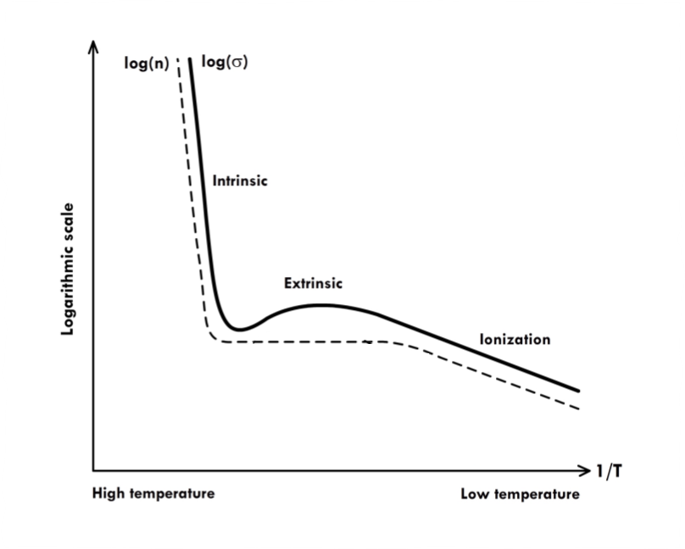
\includegraphics[width=0.8\textwidth]{Hall_temp.png}
    \caption{
    מוליכות, מוביליות וצפיפות נושאי המטען כתלות בטמפרטורה,
    לקוח מהתדריך
    \cite{Manual}.
    }
    \label{fig:conductivity_temp_theory}
\end{graph}

בטמפ' מאוד נמוכות,
נושאי המטען של החומר המסמם עוד מחוברים לאטומי
האילוח ואינם חופשיים לנוע בשריג בפס
ההולכה. עם העליה בטמפ' אטומי האילוח
יעברו יינון והאלקטרונים שלהם יעברו
לפס ההולכה. 
בתחום האקסטרינזי כל נושאי המטען של החומר המסמם יהיו מיוננים וכמות נושאי המטען בקירוב נשארת קבועה.
לבסוף, בטמפרטורות הגבוהות מסופקת למערכת מספיק אנרגיה להתגבר על הפער האנגטי של המלמ והחומר המסמם נהיה זניח.
בתחום זה המל"מ נהיה אינטרינזי והקשר בין כמות נושאי המטען לטמפרטורה נתון בנוסחא 
\ref{fig:conductivity_temp_theory}.

\begin{equ}
$$n = n_0 e^{-\frac{E_g}{2K_bT}}$$
\caption{כמות נושאי המטען כתלות בטמפרטורה עבור מל"מ אינטרינזי.}
\label{equ:n_temp_intrinsic}
\end{equ}

בניסוי זה נעבוד עם מערכת של 
\textenglish{PHYWE}-
\textenglish{Halleffect-Modul},
עם המל"מ
\textenglish{germanium}
מסוג 
\textenglish{n-type}.

\section{תוצאות}
בחלקו הראשון של הניסוי מדדנו את המתח הישר
$V$
כתלות בזרם
$I$.
התוצאות מוצגות בגרף
\ref{fig:part_0}.

\begin{graph}[ht!]
    \centering
    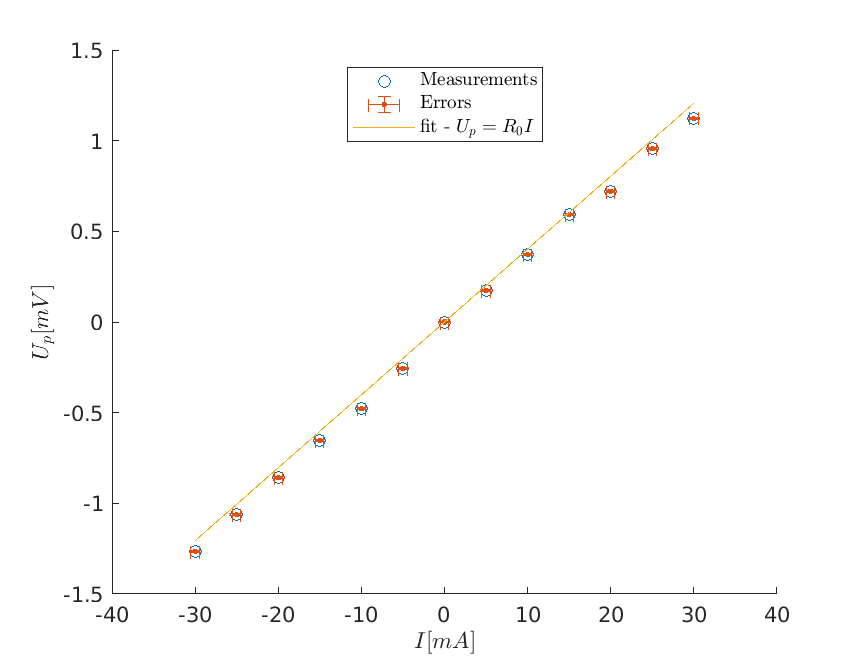
\includegraphics[width=0.8\textwidth]{part0 - R_0.png}
    \caption{המתח הישר כתלות בזרם.}
    \label{fig:part_0}
\end{graph}


לאחר מכן הפעלנו שדה מנגטי בניצב לכיוון הזרם בגודל של 
$B = (250 \pm 1) mT$ 
לשם קבלת אפקט הול. תוצאות מדידת מתח הול כתלות בזרם מוצגות בגרף
\ref{fig:part_1}.

\begin{graph}[ht!]
    \centering
    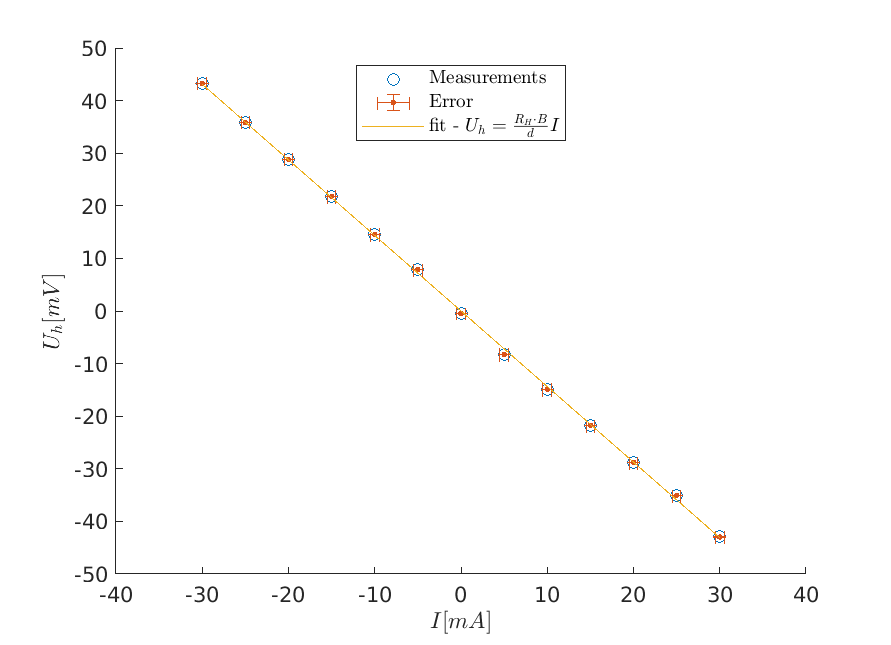
\includegraphics[width=0.8\textwidth]{part1 - R_h.png}
    \caption{מתח הול כתלות בזרם}
    \label{fig:part_1}
\end{graph}
לאחר מכן קבענו זרם קבוע של
$I = (30 \pm 1) mA$,
ושנינו את השדה המגנטי.
בגרף
\ref{fig:part_2}.
מוצגות מדידות של מתח הול כתלות בשדה המגנטי,
ובגרף
\ref{fig:part_3}.
מוצגות מדידות של המתח הישר כתלות בשדה המגנטי.

\begin{graph}[ht!]
    \centering
    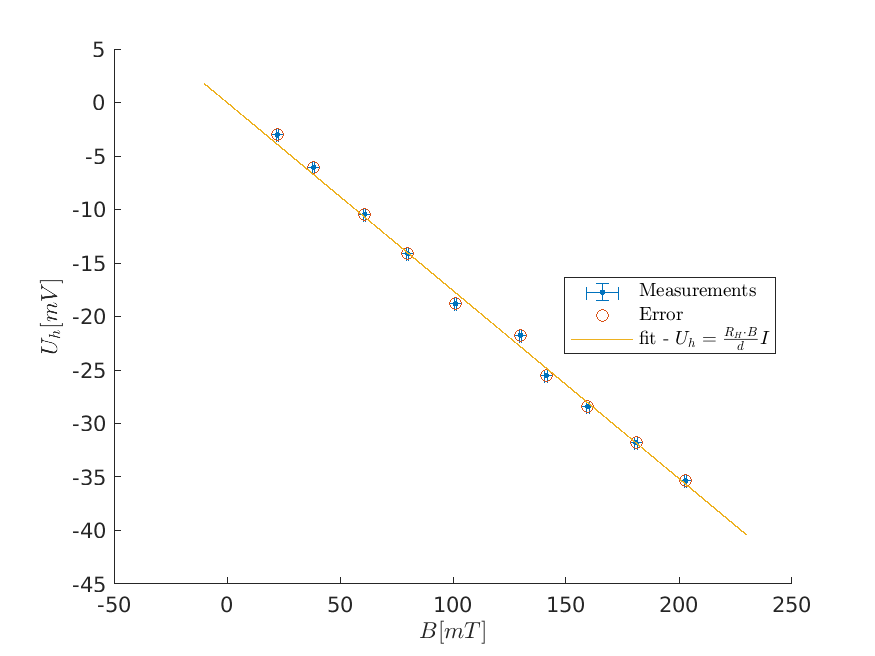
\includegraphics[width=0.8\textwidth]{part2 - R_h.png}
    \caption{מתח הול כתלות בשדה המגנטי}
    \label{fig:part_2}
\end{graph}

\begin{graph}[ht!]
    \centering
    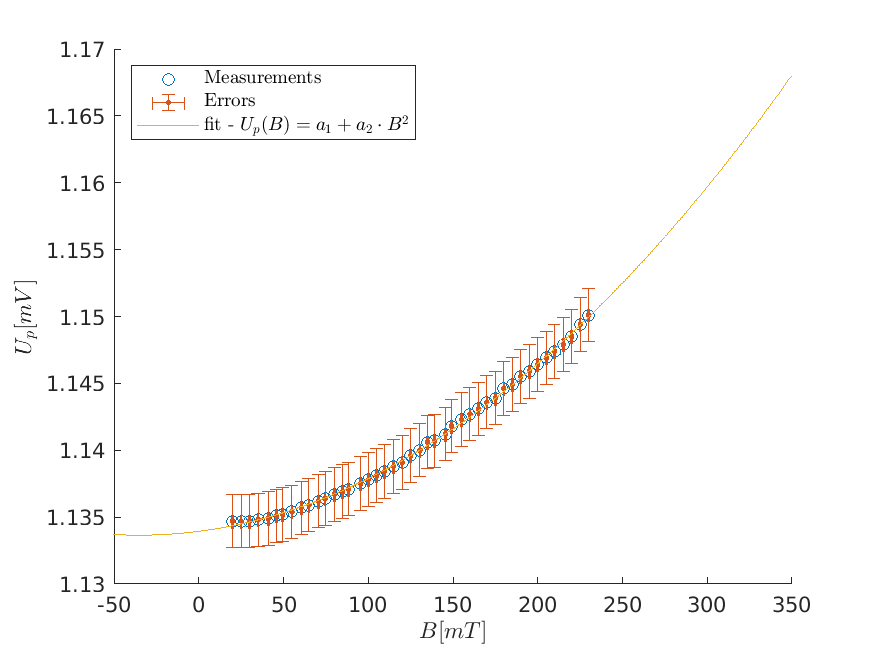
\includegraphics[width=0.8\textwidth]{part3 - B-squared relation}
    \caption{המתח הישר כתלות בשדה המגנטי}
    \label{fig:part_3}
\end{graph}
    
לבסוף מדדנו את הקשר בין המוליכות לטמפרטורה בעזרת שני מדידות :מדידת המתח הישר ומתח הול.
התוצאות מוצגות בגרפים
\ref{fig:part_4}
ו-
\ref{fig:part_5}
בהתאמה.

\begin{graph}[ht!]
    \centering
    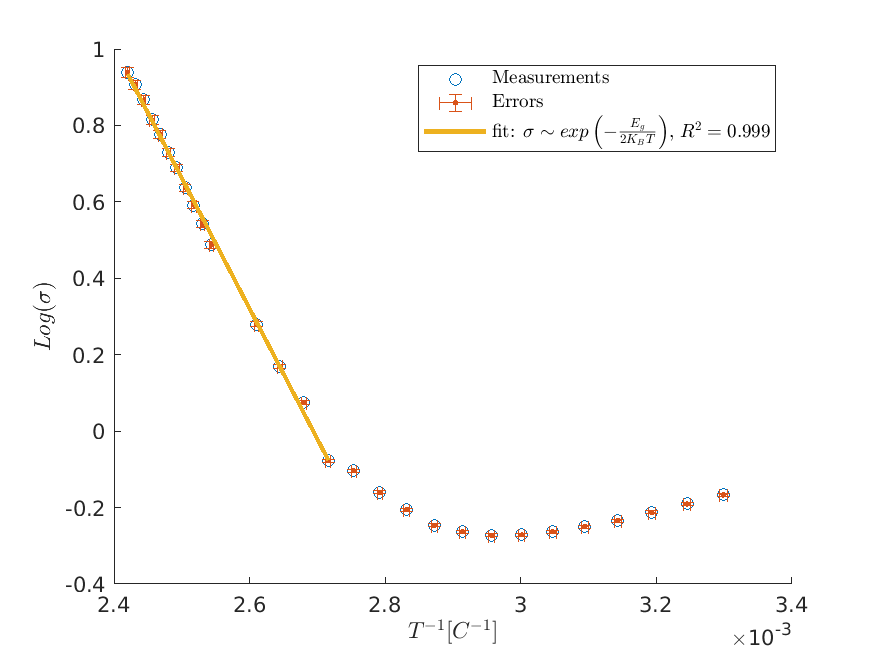
\includegraphics[width=0.8\textwidth]{part4 - E_g.png}
    \caption{מוליכות כתלות בטמפרטורה במדידת מתח ישר}
    \label{fig:part_4}
\end{graph}

\begin{graph}[ht!]
    \centering
    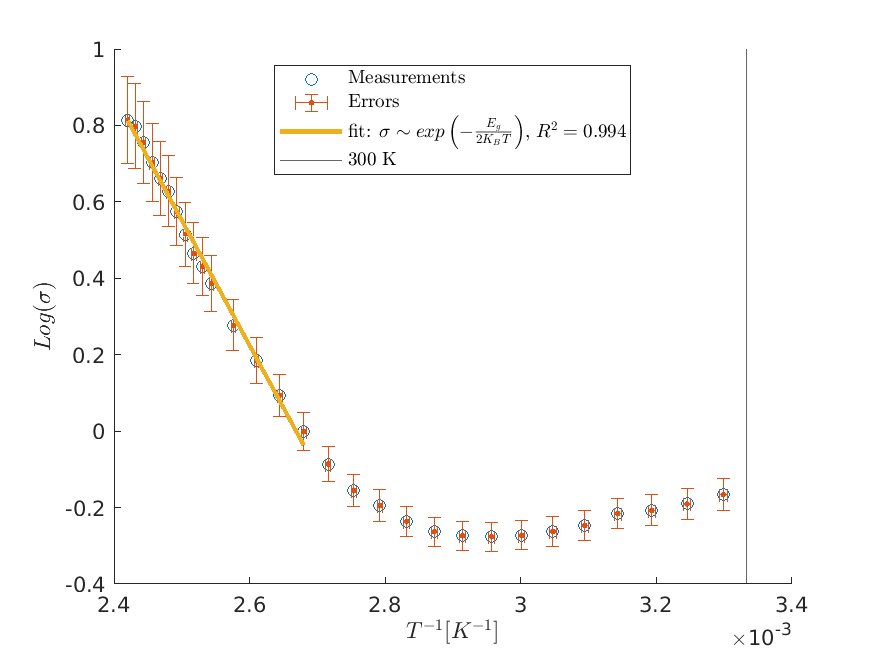
\includegraphics[width=0.8\textwidth]{part5 - E_g with magnetic field.png}
    \caption{מוליכות כתלות בטמפרטורה במדידת מתח הול}
    \label{fig:part_5}
\end{graph}



\end{document}